\chapter{Programmes Utililtaires}


Cette section d\'ecrit diff\'erents \emph{petits utilitaires}
de traitement d'images qui, bien que ne faisant pas partie
de la mise en correspondance \`a proprement parler peuvent rendre services dans
le contexte d'utilisation de MicMac, en tant que pr\'e ou
post traitements.


%-------------------------------------------------------------------
%-------------------------------------------------------------------
%-------------------------------------------------------------------

\section{G\'en\'eralit\'es}

\subsection{G\'en\'eration du binaire}

S'il n'existe pas, chaque binaire appel\'e {\tt UnUtil}, 
peut \^etre g\'en\'er\'e :

\begin{itemize}
    \item se mettre sous la directory d'installation  d'\ELISE ;
    \item taper {\tt make bin/UnUtil};
\end{itemize}

Il suffit ensuite de lancer le binaire, avec ses argument; il est
prudent de se placer sous la directory d'installation  d'\ELISE 
(certains binaires pouvant aller y chercher des ressources \`a
partir d'un chemin relatif):

\begin{itemize}
    \item {\tt bin/UnUtil arg0  arg1 \dots}
\end{itemize}


\subsection{Liste des arguments}

Chaque commande poss\`ede des arguments obligatoires et
des aguments optionnels. Les arguments obligatoires sont 
pass\'es en premiers et ils sont identifi\'es par leur
ordre de passage. Les arguments optionnels sont pass\'e
par noms, sous une suite de la forme {\tt Tag=Val}.
Ci dessous trois exemples d'utilisation de la commande 
{\tt ScaleIm} :

\begin{itemize}
    \item {\tt bin/ScaleIm Lena.tif 1.2}
    \item {\tt bin/ScaleIm Lena.tif 1.2 YScale=1.3 P0=[100,300]}
    \item {\tt bin/ScaleIm Lena.tif 1.2 Y P0=[100,300] YScale=1.3}
\end{itemize}

Les deux derni\`eres lignes sont \'equivalentes car l'ordre des
arguments optionnels n'a pas d'importance. Les types d'argument
connus et la syntaxe associ\'ee sont :


\begin{itemize}
    \item {\bf entier, r\'eel, cha\^ines de caract\`eres}, syntaxe "naturelle";
    \item {\bf  points 2D}, syntaxe {\tt [x,y]};
\end{itemize}

Il est important de n'avoir aucun blanc \`a l'int\'erieur d'un argument.

\subsection{Aide en ligne}

Pour chaque commande, un aide sommaire peut \^etre obtenue en 
tapant :

\begin{itemize}
    \item {\tt bin/UnUtil -help}
\end{itemize}

L'aide est purement syntaxique, elle donne la liste des types
des  param\`etres , ainsi que leur tag associ\'es pour les param\`etres
optionnels. Par exemple, avec la commande {\tt ScaleIm}, on
obtiendra :

\begin{verbatim}
bin/ScaleIm  -help
*****************************
*  Help for Elise Arg main  *
*****************************
Unamed args :
  * string
  * REAL
Named args :
  * [Name=Out] string
  * [Name=YScale] REAL
  * [Name=Sz] Pt2dr
  * [Name=P0] Pt2dr
\end{verbatim}
\label{UTILBIN:HELP}


%-------------------------------------------------------------------
%-------------------------------------------------------------------
%-------------------------------------------------------------------

\section{L'utilitaire  de changement d'echelle {\tt ScaleIm}}

\subsection{Fonctionnalit\'es}

Cet utilitaire permet de calculer, \`a partir d'un fichier image,
une m\^eme image \`a une \'echelle diff\'erente.  Elle fonctionne
aussi bien en agrandissement qu'en r\'eduction. En agrandissement,
c'est un interpolateur bicubique classique qui est utilis\'e
(avec le param\`etre $-0.5$ qui interpole rigoureusement les
fonctions lin\'eaires). En r\'eduction, c'est un bicubique 
sans valeur n\'egative (param\`etre $0.0$,avec une transition
continue pour les \'echelles entre $1$ et $1.5$) qui est utilis\'e,
apr\`es avoir \'et\'e  dilat\'e du facteur de r\'eduction

Par d\'efaut, le calcul est fait sur toute l'image, mais un
cliping est possible.

Soit $S^x$ et $S^y$ les facteur de changement d'\'echelle et
$P_0$ une origine, la radiom\'etrie de  l'image $I^{out}$ est
d\'efinie \`a partir de celle de l'image d'entr\'ee $I^{in}$
par :

\begin{equation}
   I^{out}(x,y) = I^{in}(P_0^x + S^x * x,P_0^y + S^y * y)
   \label{EQ:SCALE:IM}
\end{equation}

\subsection{Param\`etres}

La liste des arguments a \'et\'e donn\'ee comme exemple de la
section~\ref{UTILBIN:HELP}:

\begin{itemize}
   \item le premier argument est le nom du fichier image en entr\'ee;

   \item le deuxi\`eme argument est le facteur de changement d'\'echelle,
          comme l'indique la formule~\ref{EQ:SCALE:IM} un facteur S avec  $S<1$
          correspond \`a un aggrandissement;

   \item le param\`etre optionnel {\tt Out}   indique le nom du fichier
         de sortie, s'il est omis un nom est calcul\'e \`a partir
          du fichier d'entr\'ee selon la transformation r\'eguli\`ere
          {\tt .*\verb|\|.tif} donne {\tt \$1\_Scaled\verb|\|.tif};

   \item le param\`etre optionnel {\tt YScale} permet de donner le changement
         d'\'echelle en $Y$ (par d\'efaut \'egal \`a S); 

   \item le param\`etre optionnel {\tt Sz} permet de sp\'ecifier la taille
         de l'image sur laquelle il faut effectuer la transformation (par
         d\'efaut le maximum, donc toute l'image quand $P^0=(0,0)$; 

   \item le param\`etre optionnel {\tt P0}  , correspond au $P_0$ de
          la formule~\ref{UTILBIN:HELP}, il d\'efinit donc l'origine  "haut-gauche"
          de la portion d'image \`a laquelle est appliqu\'ee la transformation;
          par d\'efaut $P_0=[0,0]$.
\end{itemize}

\subsection{Evolutions possibles}

Il serait possible assez facilement de pouvoir  param\'etrer 
totalement le noyau de convolution \`a condition qu'il reste s\'eparable.


%-------------------------------------------------------------------
%-------------------------------------------------------------------
%-------------------------------------------------------------------

\section{L'utilitaire d'ombrage {\tt GrShade}}

\subsection{Fonctionnalit\'es}

Cette utilitaire part d'un image assimil\'ee \`a un relief
$z=f(x,y)$ (par exemple un r\'esultat de MicMac) et calcule 
son \emph{ombrage} d\'efini comme la portion de ciel visible.
Cet ombrage a la caract\'eristique de mettre en relief
les d\'efaut de la corr\'elation. Ce n'est donc
pas toujours l'outil ad\'equat pour comprendre
le relief r\'eel, mais c'est souvent un outil assez pratique
pour juger de la qualit\'e d'un r\'esultat de corr\'elation.

Pour effectuer le calcul de la portion de ciel visible avec
une complexit\'e acceptable, le programme  discr\'etise
les directions du plan sur $N$ valeurs et effectue un balayage
sur ces $N$ directions; pour chaque direction, on a un signal $1D$ 
et le probl\`eme revient au calcul en chaque point de la pente 
du rayon  tangent au  point d'ombrage; pour ce probl\`eme, un algorithme
r\'ecursif rapide permet de faire le calcul en temps lin\'eaire.

Gloablement, le temps de calcul est donc en $N^{pix}*N^{dir}$ ou
$N^{pix}$ est le nombre de pixels de l'image et $N^{dir}$ est le
nombre  sur lequel on choisit de discr\'etiser les directions
du plan.


\subsection{Param\`etres}

Il y un seul param\`etre obligatoire qui indique le nom du fichier
image en entr\'ee. 

Les principaux param\`etres optionnels sont les suivants :

\begin{itemize}
   \item {\tt \bf FZ :} \emph{(real)}  d\'efinit le pas en $z$ par lequel
         est multipli\'e le relief avant d'\^etre ombr\'e, vaut $1.0$
         par d\'efaut; peut \^etre n\'egatif;

   \item {\tt \bf Out :} \emph{(string)}  nom du fichier de sortie, s'il n'est 
         pas sp\'ecifi\'e il vaut {\tt InputShade.tif}  (en
         supposant que l'entr\'ee s'apelle  {\tt Input.tif} );

   \item {\tt \bf Anisotropie :} \emph{(real)} s'il vaut $0$, on a
         un ombrage isotrope (toutes les directions sont \'equivalentes);
         plus il est proche de 1, plus on fait jouer un r\^ole privil\'egi\'e
         aux directions proche du "nord"; il doit obligatoirement \^etre
         compris entre $0$ et $1$; sa valeur par d\'efaut est $0.95$;

   \item {\tt \bf Dequant :} \emph{(int)}  , les MNT sont souvent quantifi\'es,
         c'est le cas de ceux produits par MicMac; une fois ombr\'e le MNT
         quantifi\'e a un aspect relief en plateau (type rizi\`ere) qui
         peut \^etre consid\'er\'e comme un d\'esagr\'ement; si ce
         param\`etre est $\neq 0$, un algorithme de "d\'equantification"
         est appliqu\'e en amont de l'ombrage (algorithme de type interpolation
         lin\'eaire), sa valeur par d\'efaut est $0$;

   \item {\tt \bf HypsoDyn :} \emph{(real)}  ,{\tt \bf HypsoSat :}

\end{itemize}

Les param\`etres optionnels suivants sont d'usage moins courant:



\begin{itemize}
   \item {\tt \bf Visu :} \emph{(int)}  indique de mani\`ere bool\'eenne 
         s'il y a visualisation en temps r\'eel du calcul,  vaut $0$ 
         par d\'efaut;
         
   \item {\tt \bf P0 :} \emph{(Pt2di)} , {\tt \bf Sz :} \emph{(Pt2di)} 
         d\'efinissent la bo\^ite englobante sur laquelle est effectu\'e
         le calcul;

   \item {\tt \bf NbDir :} \emph{(int)}  nombre de valeurs sur lequel sont
         discr\'etis\'ees  les directions du cercle, correspond \`a un
         compromise "qualit\'e/temps de calcul" (valeur par d\'efaut 20);
         
   \item {\tt \bf Brd :} \emph{(int)} souvent les valeur en bord d'images
         sont bruit\'ees (voir sans significations), si ce sont des valeurs
         \'elev\'ees elles ont une forte influence sur l'ombrage; ce 
         param\`etre permet de mettre sur un bord de taille {\tt Brd}
         la valeur minimale du fichier afin que le bord n'influence
          pas l'ombrage, vaut $0$ par d\'efaut;

   \item {\tt \bf TypeMnt :} \emph{(int)}, {\tt \bf TypeShade :} \emph{(int)},
         type des images temporaires utilis\'ees pour le calcul temporaire;
         peut valoir {\tt u\_int1,int1,u\_int2,int2,real4}, 
         par d\'efaut vaut {\tt real4}; permet \'eventuellement 
         d'\'economiser de la m\'emoire, usage d\'econseill\'e;
\end{itemize}


\subsection{Evolutions possibles}

L'algorithme permet, sans changer de compl\'exit\'e de
prendre n'importe quelle fonction d'illumination (densit\'e
de lumi\`ere/st\'eradian en chaque point de la sph\`ere).
Il serait possible de laisser l'utilisateur sp\'ecifier sa propre
fonction, ce qui pourrait avoir un int\'er\^et dans l'utilisation
pour des simulation "physique".

%-------------------------------------------------------------------
%-------------------------------------------------------------------
%-------------------------------------------------------------------

\section{L'utilitaire lumi\`ere rasante {\tt LumRas}}

\subsection{G\'en\'eralit\'es}
Cet utilitaire permet de fusionner une image ma\^itresse en \'eclairage diffus avec des images esclaves en \'eclairage rasant. Le traitement permet de faire ressortir le micro-relief de certaines surfaces\footnote{Voir la th\`ese de Maryam Saaman : \url{https://tel.archives-ouvertes.fr/tel-01547923}}. L'outil {\tt LumRas} doit \^etre utilis\'e apr\`es {\tt Tapioca} pour qu'il puisse aligner correctement les images entre elles.

\subsection{Liste des arguments}
Cette commande attend deux arguments obligatoires :
\begin{itemize}
\item le nom de l'image ma\^itresse,
\item et l'expression r\'eguli\`ere des images esclaves.
\end{itemize}
Un argument optionnel ({\tt Masq=}) permet d'indiquer le suffixe du masque de la zone \`a calculer saisi sur l'image ma\^itresse (par d\'efaut {\tt Masq} suite \`a l'utilisation de {\tt SaisieMasq}).

\begin{verbatim}
LumRas

Unamed args :
  * string :: {Master image}
  * string :: {Raking light images pattern}
Named args :
  * [Name=Masq] string :: {Master image mask postfix (Def=_Masq)}

\end{verbatim}

\subsection{Exemple}
Dans cet exemple, une pi\`ece de monnaie a \'et\'e photographi\'ee en condition d'\'eclairage naturel, puis cinq photographies en lumi\`ere rasante ont \'et\'e acquises.

\begin{figure}[h!]
\centering
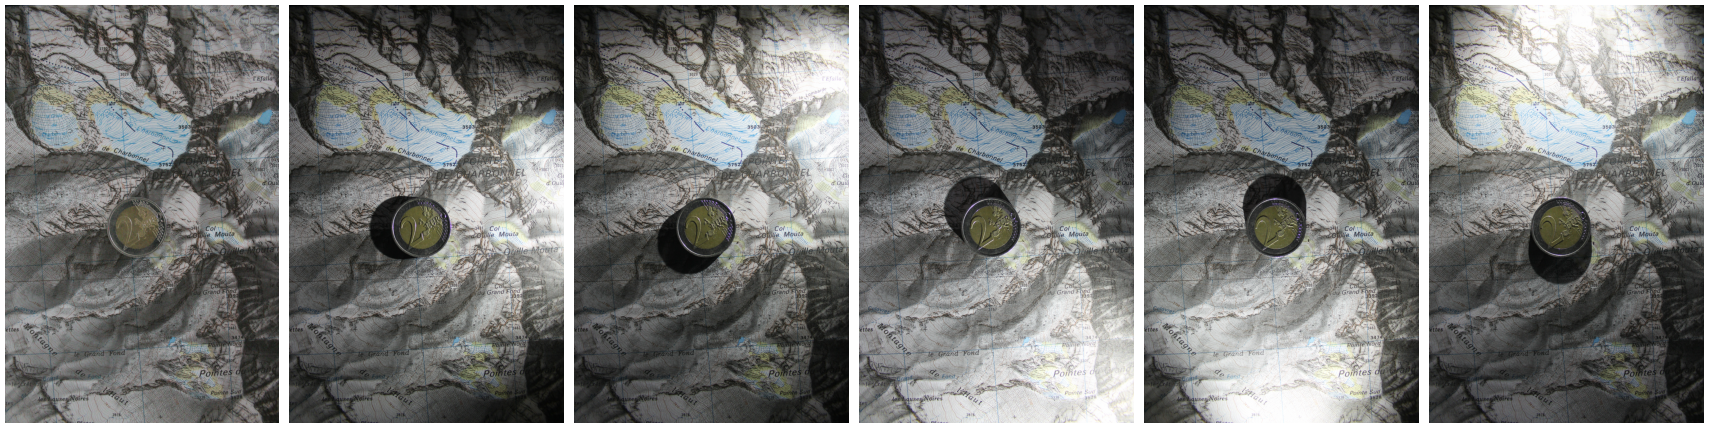
\includegraphics[width=\textwidth]{FIGS/LumRas/LumRasPanel.png}
\caption{L'image ma\^itresse et les images esclaves}
\end{figure}

\begin{figure}[h!]
\centering
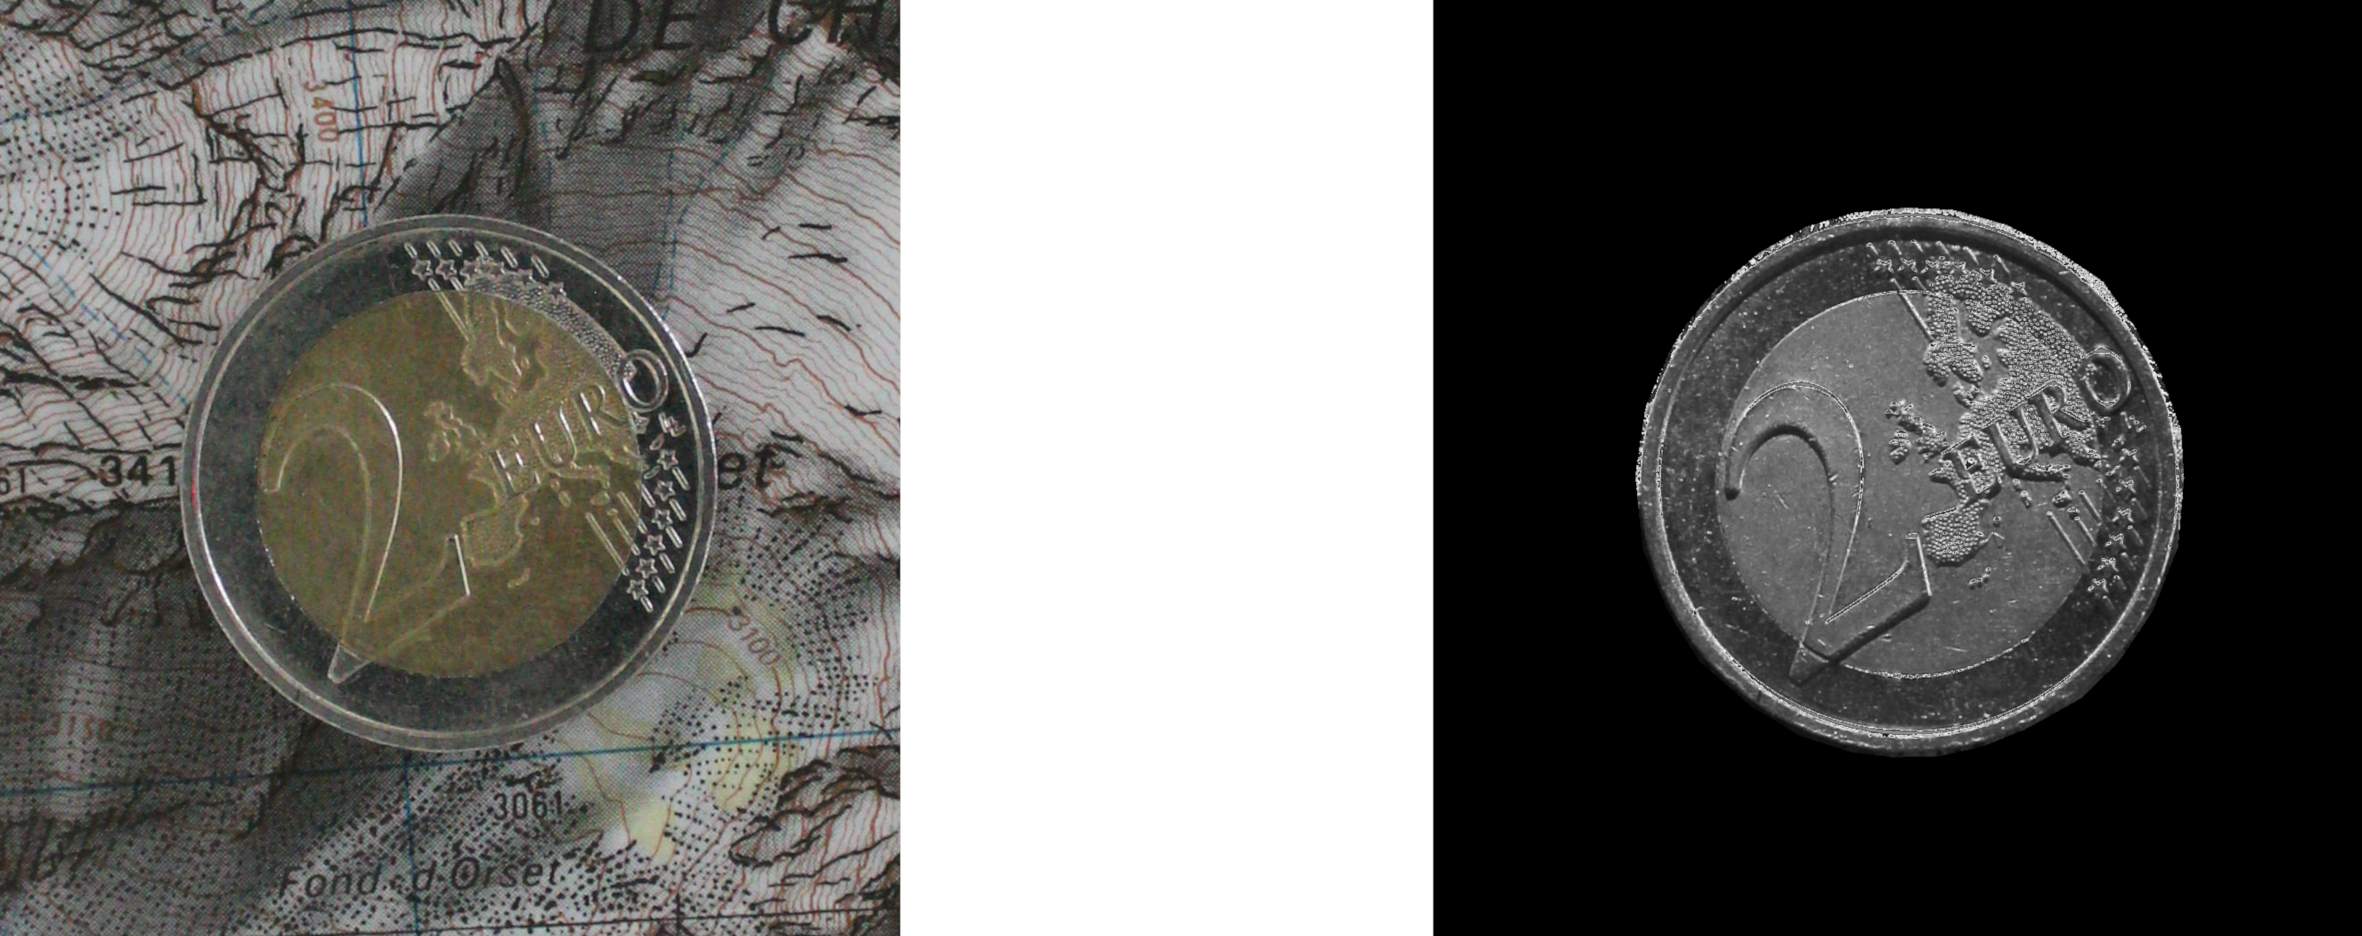
\includegraphics[width=0.8\textwidth]{FIGS/LumRas/LumRasExample.png}
\caption{D\'etail de l'image d'origine et de l'image calcul\'ee}
\end{figure}

%-------------------------------------------------------------------
%-------------------------------------------------------------------
%-------------------------------------------------------------------

\section{L'utilitaire de d\'equantification  {\tt Dequant}}

%-------------------------------------------------------------------
%-------------------------------------------------------------------
%-------------------------------------------------------------------

\section{L'utilitaire d'information sur un fichier tiff {\tt tiff\_info}}


%-------------------------------------------------------------------
%-------------------------------------------------------------------
%-------------------------------------------------------------------

\section{L'utilitaire  de test des expression r\'eguli\`ere {\tt test\_regex}}


%-------------------------------------------------------------------
%-------------------------------------------------------------------
%-------------------------------------------------------------------


\section{SupMntIm to superpose image and DTM}


bin/SupMntIm $A_1$ $A_2$

\begin{itemize}
    \item $A_1$ = Absolute Name of Image
    \item $A_2$ = Absolute Name of Mnt
    \item {\tt DynCoul} , dynamique of colour, real, $Def=1.0$
    \item {\tt CDN} , generate level curve ?  Boolean, $Def=0$
\end{itemize}






